\chapter{Loop Optimizations}

Formele definitie van een lus in een CFG: verzameling knopen $S$ met daarin een header $h$ met volgende eigenschappen:
\begin{itemize}
	\item Vanuit elke knoop in $S$ is er een pad dat naar $h$ leidt.
	\item Vanuit $h$ is er een pad naar elke knoop in $S$.
	\item Er is geen enkele andere knoop buiten $S$ die naar een knoop in $S$ wijst, behalve $h$.
\end{itemize}

\begin{figure}[ht]
	\centering
	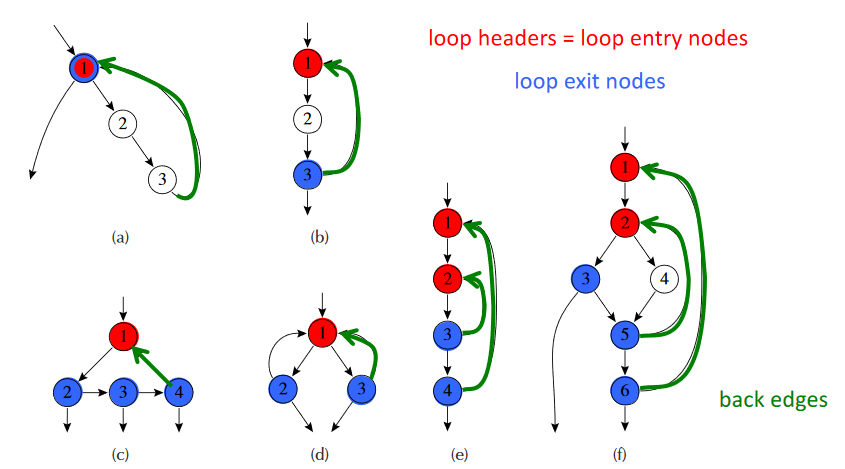
\includegraphics[width=\textwidth]{loops}
	\caption{Voorbeelden van lussen; in elk geval is $1$ de header knoop.}
	\label{fig:loops}
\end{figure}

De knopen in een lus vormen een \textit{strongly connected component}: vanuit één knoop in de lus kan elke andere knoop in de lus bereikt worden. De \textbf{back edge} is de verbinding die een knoop naar de header verbindt

Reduceerbaarheid = niet te kennen. Enkel weten dat lussen volledig overlappen of helemaal niet. Ze kunnen niet deels overlappen.

\section{Dominators}
\begin{itemize}
	\item Veronderstel 1 startknoop $s_0$ van de $CFG$.
	\item Knoop $d$ domineert knoop $n$ als elk pad van $s_0$ naar $n$ door $d$ gaat.
	\item Eenvoudig berekenen met data flow analyse. 
	$$D[s_0] = \{s_0\}, \qquad D[n] = \{n\} \cup \bigg(\bigcap_{p \in pred[n]} D[p] \bigg) \quad \hbox{for } n \neq s_0$$
	Aangezien de intersectie berekend wordt moet dit algoritme geïnitialiseerd worden met maximale sets.
	\item In plaats van data  flow analyse kan ook de dominator tree opgesteld worden. De dominator set van een knoop is dan de opeenvolging van ouderknopen.
\end{itemize}

Eigenschappen van een dominator:
\begin{itemize}
	\item Transitief: $a$ dom $b$ en $b$ dom $c$ $\rightarrow a$ dom $c$.
	\item Als $e$ dom $n$ en $d$ dom $n$, dan $e$ dom $d$ of $d$ dom $e$.
	\item Elke knoop $n$ heeft een unieke immediate dominator \texttt{idom($n$)}.
	\begin{itemize}
		\item \texttt{idom($n$)} $\neq n$.
		\item \texttt{idom($n$)} domineert $n$.
		\item \texttt{idom($n$)} domineert geen andere dominator van $n$.
	\end{itemize}
\end{itemize}

De graaf waarin elke knoop $n$ van de CFG in voorkomt en waarbij er een verbinding is tussen $n$ en \texttt{idom($n$)} wordt een \textbf{dominator tree} genoemd (figuur \ref{fig:dominator_tree}).

\begin{figure}[ht]
	\centering
	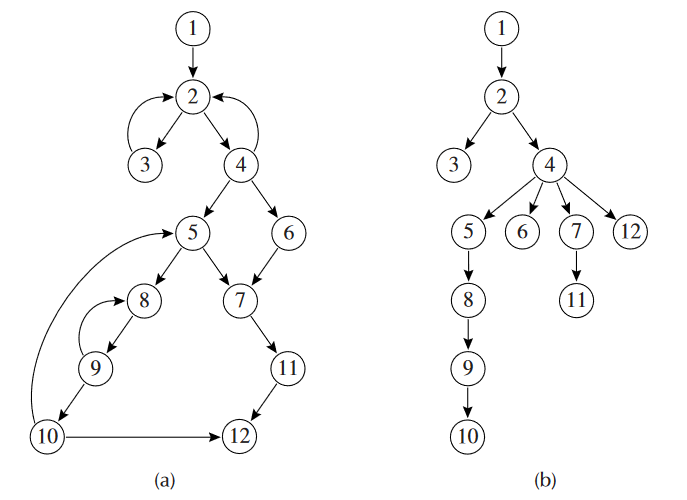
\includegraphics[width=0.7\textwidth]{dominator_tree}
	\caption{(a) Een CFG; (b) de corresponderende dominator tree.}
	\label{fig:dominator_tree}
\end{figure}

\subsection{Header loops}
\begin{itemize}
	\item Een \textbf{natuurlijke loop} van een \textbf{back edge} $n \rightarrow h$, waarbij $h$ dom $n$, is de verzameling knopen $x$ zodat $h$ elke $x$ domineert en er een pad is van $x$ naar $n$ zonder $h$.
	\item Een header $h$ kan header zijn van meerdere lussen.
	\item Loops kunnen genest zijn.
	\item Een loop-nest tree geeft aan welke knopen op welk loopniveau ze zitten. Voor een flow-graaf $G$ kan deze als volgt opgebouwd worden:
	\begin{itemize}
		\item Bepaal de dominators van $G$.
		\item Bouw de dominator tree.
		\item Zoek alle natuurlijke loops, en dus ook alle loop-header knopen.
		\item Voor elke loop header $h$, voeg de natuurlijke loops van $h$ samen in een enkelvoudige loop, loop[h].
		\item Bouw de loop-nest tree, zodat $h_1$ boven $h_2$ is als $h_2$ zich bevindt in $loop[h_1]$.
	\end{itemize}
	\begin{figure}[ht]
		\centering
		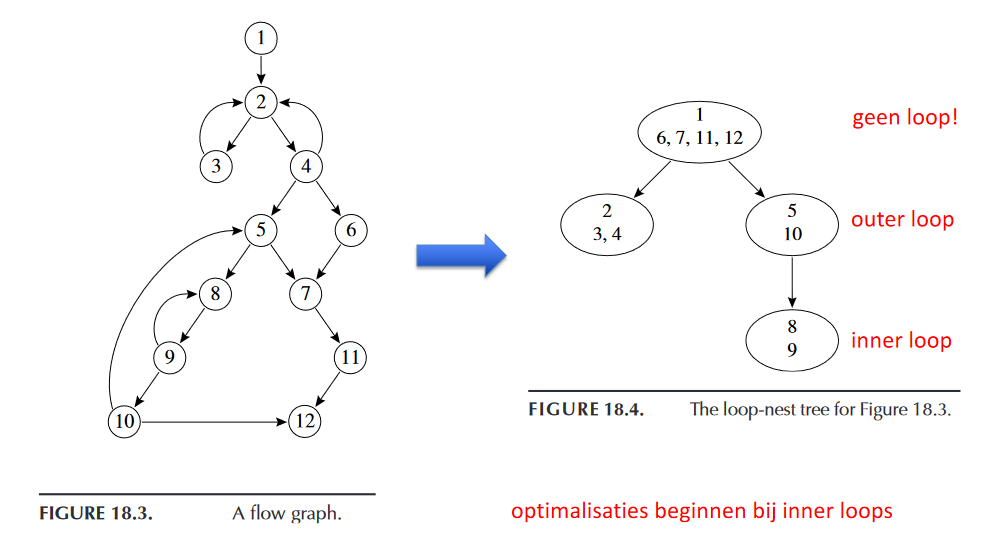
\includegraphics[width=0.75\textwidth]{loop_nest_tree}
		\caption{Een flow-graph en de bijhorende loop-nest tree.}
		\label{fig:loop_nest_tree}
	\end{figure}

\end{itemize}

\subsection{Loop preheader}
\begin{itemize}
	\item Algemene code die voor een lus moet uitgevoerd worden.
	\item Resulteert in een extra knoop $p$, met de verbinding $p \rightarrow h$.
	\item Handig als er meerdere paden naar de header van de lus zijn.
\end{itemize}



\section{Loop Invariant Computations}
\begin{itemize}
	\item Berekeningen die altijd dezelfde waarde hebben kunnen eventueel buiten de lus geplaatst worden. 
	\alert Soms is het herberekenen wel beter dan registers te gebruiken.
	\item Een definitie $d : t \leftarrow a_1 \oplus a_2$ is loop-invariant als voor elke $a_i$:
	\begin{itemize}
		\item $a_i$ een constante is;
		\item alle definities van $a_i$ die $d$ bereiken zich buiten de lus bevinden;
		\item of de enige definitie van $a_i$, die $d$ bereikt, loop-invariant is.
	\end{itemize}
	\item Stel dat $d : t \leftarrow a_1 \oplus a_2$ loop-invariant is, dan mag deze buiten de lus (in de loop preheader) geplaatst worden op drie voorwaarden:
	\begin{enumerate}
		\item Het is de enige definitie van $t$ in de lus,
		\item $d$ domineert elke loop exit waarbij $t$ live-out is,
		\item $t$ is niet live-out bij de preheader.
	\end{enumerate}
\end{itemize}

\begin{figure}[ht]
	\centering
	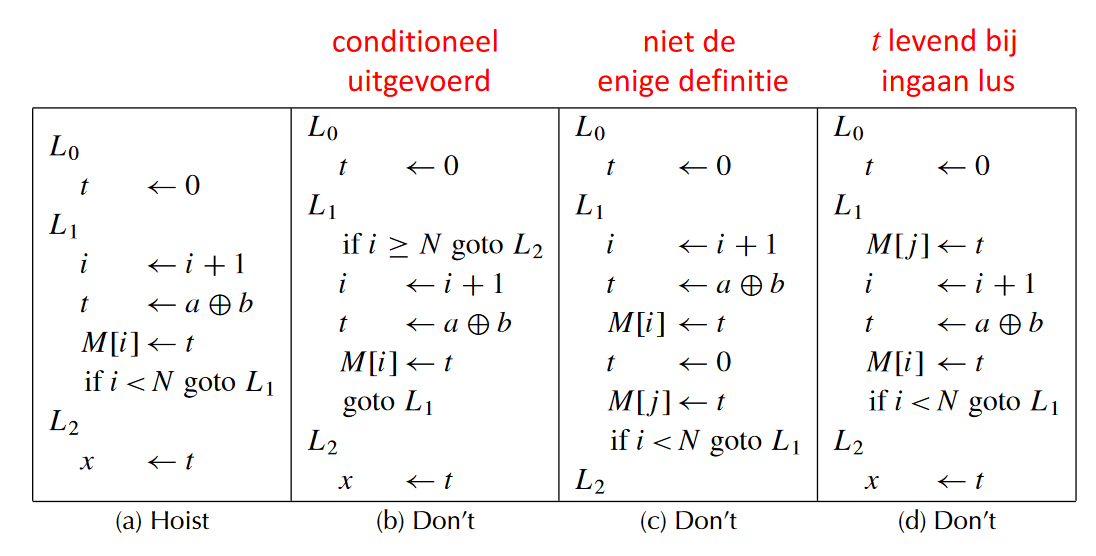
\includegraphics[width=\textwidth]{hoisting}
	\caption{Voorbeelden voor de operatie $t \leftarrow a \oplus b$ Slechts als de drie criteria voldaan zijn mag de operatie buiten de lus geplaatst wordt, en is enkel van toepassing op (a).}
	\label{fig:hoisting}
\end{figure}

Oppassen met side-effects: exceptions, pointer dereferencing

\section{Inductieveranderlijken}
\begin{itemize}
	\item Een inductieveranderlijke is een variabele dat geïncrementeerd of gedecrementeerd wordt met een vaste waarde bij elke iteratie van een lus.
	\item Twee soorten:
	\begin{enumerate}
		\item \textbf{Basisinductieveranderlijke}: Een variabele $i$ is een basisinductieveranderlijke in een lus $L$ met header $h$ als de enige definities van $i$ in $L$ één van volgende vormen heeft, met $c$ een constante:
		\begin{itemize}
			\item $i \leftarrow i + c$
			\item $i \leftarrow i - c$
		\end{itemize} 
		\item \textbf{Afgeleide inductieveranderlijke}: Een varaiabele $k$ is een afgeleide inductieveranderlijke in lus $L$ als:
		\begin{enumerate}
			\item Er slechts één definitie van $k$ binnen $L$ is, en één van de volgende vormen heeft:
			\begin{itemize}
				\item $k \leftarrow j \cdot c$
				\item $k \leftarrow j + d$
			\end{itemize}
			Hierbij is $j$ een inductievariabele en $c$, $d$ zijn loop-invariant.
			\item en als $j$ een afgeleide inductieveranderlijke is in de familie $i$, dan:
			\begin{enumerate}
				\item de enige definitie van $j$ dat $k$ bereikt bevindt zich in $L$,
				\item en er is geen definitie van $i$ op elk pad tussen de definitie van $j$ en $k$.
			\end{enumerate}
		\end{enumerate}
	\end{enumerate}
\end{itemize}



\section{Loop unrolling}
\begin{itemize}
	\item Gegeven een lus $L$ met header $h$ en back edges $s_i \rightarrow h$, de loop kan dan gekopieerd worden:
	\begin{enumerate}
		\item Kopieer alle knopen om een lus $L'$ te maken met header $h'$ en back edges $s_i' \rightarrow h'$.
		\item Verander alle back edges in $L$ van $s_i \rightarrow h$ naar $s_i \rightarrow h'$.
		\item Verander alle back edges in $L'$ van $s_i' \rightarrow h$ naar $s_i' \rightarrow h$.
	\end{enumerate}
\end{itemize}